\documentclass[border=10px]{standalone}
\usepackage{tikz}
\usetikzlibrary{patterns}
\usetikzlibrary{shapes.arrows}
\usepackage{amssymb}
\usetikzlibrary{calc}
\usepackage{verbatim}
\usepackage[swedish]{babel}
\begin{document}
	
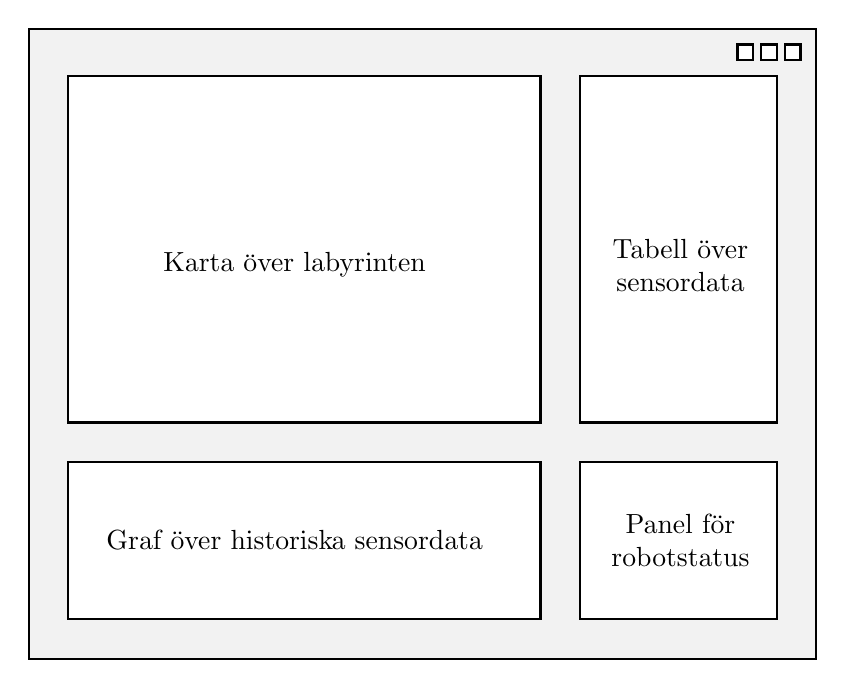
\begin{tikzpicture}[scale=1,rotate=0]
		
	%Frame
	\draw[thick, draw=black, fill=gray!10] (0,0) rectangle (10,8);

	%Exit and minimize
	\draw[thick, draw=black, fill=white] (9.0,7.6) rectangle (9.2,7.8);
	\draw[thick, draw=black, fill=white] (9.3,7.6) rectangle (9.5,7.8);
	\draw[thick, draw=black, fill=white] (9.6,7.6) rectangle (9.8,7.8);
	
	%Map
	\draw[thick, draw=black, fill=white] (0.5,3) rectangle (6.5,7.4);
	\draw  node[left, align=center, text width=5cm] at (6,5) {Karta över labyrinten};
	
	%Table
	\draw[thick, draw=black, fill=white] (7, 3) rectangle (9.5,7.4);
	\draw  node[left, align=center, text width=2cm] at (9.4,5) {Tabell över sensordata};
	
	
	%Graph
	\draw[thick, draw=black, fill=white] (0.5,0.5) rectangle (6.5,2.5);
	\draw  node[left, align=center, text width=5cm] at (6,1.5) {Graf över \mbox{historiska} sensordata};
	
	%Buttons
	\draw[thick, draw=black, fill=white] (7,0.5) rectangle (9.5,2.5);
	\draw  node[left, align=center, text width=2cm] at (9.4,1.5) {Panel för robotstatus};
	
	
	\end{tikzpicture}
	
\end{document}